El modelo empleado es una arquitectura recurrente de inferencia de máscaras, basada en una LSTM que recibe la magnitud de la STFT de la mezcla y predice una máscara por fuente. Estas máscaras se aplican sobre la magnitud de la mezcla para obtener las magnitudes estimadas de cada \textit{stem}. En la Figura \ref{fig:LSTM} se muestra un ejemplo de una arquitectura LSTM.

\begin{figure}[H]
    \begin{center}
    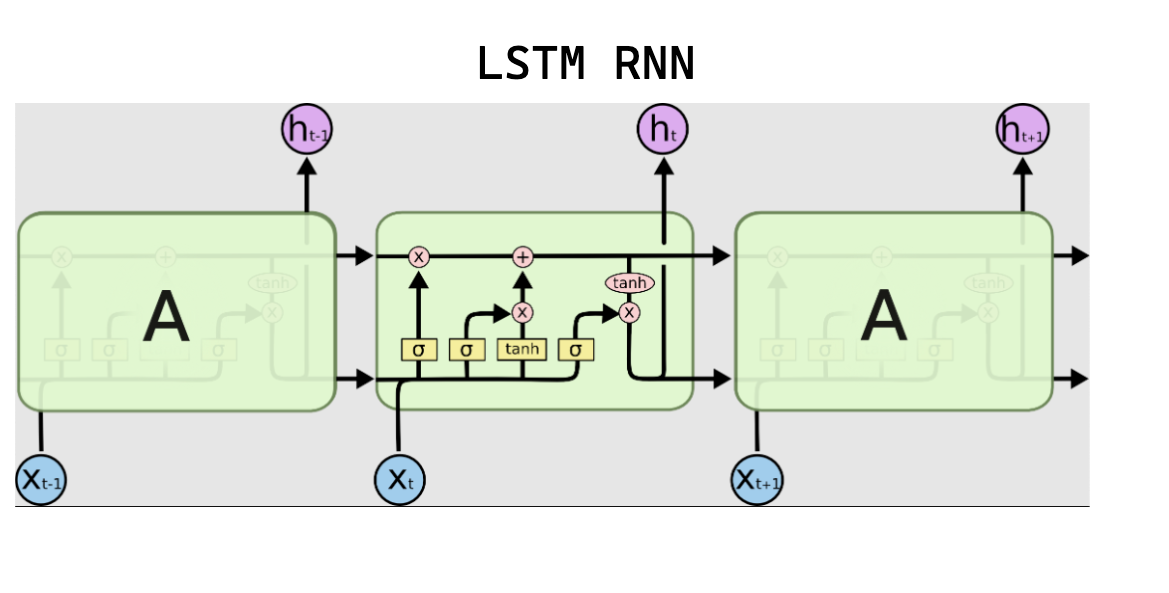
\includegraphics[width=0.7\textwidth]{commons/Fig9.png}
    \caption{Ejemplo de una arquitectura RNN-LSTM}
    \label{fig:LSTM}
    \cite{rafii18}
    \end{center}
\end{figure}


La arquitectura LSTM es comúnmente utilizada en separación de fuentes por su capacidad de retener información, de olvidarla, de análisis secuencial y de mantener contexto pasado y futuro de la información actual para el caso de una LSTM bidireccional.
Una LSTM procesa una secuencia  de información mediante pasos a través de celdas, normalmente palabras, sonidos o datos en general que se definen a lo largo de un eje temporal.
Una celda LSTM mantiene un estado de celda \(c_t\) que transporta memoria temporal y un estado oculto \(h_t\) usado como salida. Las puertas de olvido, entrada y salida regulan qué información se conserva, incorpora y expone en cada instante.

En el contexto del proyecto el sistema introduce al modelo la interpretación en secuencia temporal de un espectrograma (es decir, la magnitud de la STFT de la entrada), a partir del cual, la LSTM procesa esta secuencia para estimar máscaras que aplicadas sobre
la mezcla original producen una pista fuente. A lo largo del proyecto ha habido modificaciones de los parámetros utilizados y la configuración final se puede ver en la Tabla \ref{tab:parametros_modelo}.

\begin{table}[H]
    \centering
    \footnotesize
    \renewcommand{\arraystretch}{1.15}

    \begin{tabularx}{\textwidth}{
        >{\raggedright\arraybackslash}p{0.25\textwidth}
        >{\raggedright\arraybackslash}X
        >{\raggedright\arraybackslash}p{0.20\textwidth}
    }
        \hline

        \textbf{Parámetro} & \textbf{Definición} & \textbf{Valor} \\

        \hline

        Tamaño de ventana STFT &
        Número de muestras de la onda de entrada sobre las que se aplica la transformada de Fourier de tiempo corto. &
        512 muestras \\

        Salto STFT &
        Separación entre una ventana y la consecutiva. &
        128 muestras \\

        Tipo de ventana &
        Forma de la ventana utilizada en la STFT. &
        \texttt{sqrt\_hann} \\

        Número de bins de frecuencia &
        Número de frecuencias únicas resultantes de una FFT de 512 puntos sobre una señal real. &
        257 \\

        Canales de entrada &
        Número de canales de audio procesados por la red. &
        1, mono \\

        Tipo de red recurrente &
        Red encargada de modelar las dependencias temporales entre espectros consecutivos. &
        LSTM \\

        Número de capas recurrentes &
        Número de capas LSTM utilizadas. &
        1 \\

        Tamaño oculto &
        Número de unidades ocultas por dirección en cada capa LSTM. &
        50 \\

        Bidireccional &
        Determina si la LSTM analiza tanto el contexto pasado como el futuro. &
        Sí \\

        Dropout &
        Probabilidad de desactivar aleatoriamente unidades durante el entrenamiento. &
        0.0 \\

        Activación de salida &
        Función que transforma las salidas en valores comprendidos entre cero y uno. &
        Sigmoid \\

        Salidas en 2 stems &
        Fuentes estimadas en la configuración de dos stems. &
        vocals, accompaniment \\

        Salidas en 4 stems &
        Fuentes estimadas en la configuración de cuatro stems. &
        vocals, bass, drums, other \\

        \hline
    \end{tabularx}

    \caption{Configuración arquitectónica de parámetros utilizada en los entrenamientos finales del proyecto.}
    \label{tab:parametros_modelo}
\end{table}

